%===========================================================
\chapter{Persistence and Checkpoints}
%===========================================================

\section{Format}
Checkpoints are JSON documents with format \code{vikasa}, \textbf{version 3}. They
store the resolved configuration, seed, tick, the NumPy PCG64 bit-generator state,
all creatures (genome, haplotypes, temperament, energy, injury, age, starvation
counter, current action, drives, utilities, targets, home-range and migration
state, satisfaction components, alpha status, belief, and with climate forcing the
thermal optimum and stress), resources, lineage, the environment and event
history, the culture ledger, metrics (including the last 512 birth cohorts), the
optional habitat grids and ledgers, intervention records, cumulative counters and
the fractional food-spawn accumulator.

\section{Atomic saving}
\code{save\_checkpoint} serialises the payload, rejects non-finite values (NaN or
infinity are refused rather than written as invalid JSON), writes a temporary
sibling file, flushes and syncs it, and atomically replaces the destination. An
interrupted save therefore never leaves a half-written checkpoint.

\section{Loading, migration and validation}
\code{load\_checkpoint} accepts versions 1, 2 and 3. Versions 1 and 2 are migrated
in memory: missing behaviour and home-range fields receive defaults, and
home radii are sampled deterministically per creature. Loading never rewrites the
source file; saving a migrated run writes version 3. Version 3 is strict:
required fields must be present, IDs and references must be JSON integers (booleans
and floats are rejected), and invariants must hold. The loader rejects malformed
habitat grids, impossible initialisation totals, unadvanced dynamic fluxes,
unbalanced reservoir ledgers, persisted birth histories that are out of order or
violate the Price identity, and unsupported versions. All failures raise
\code{CheckpointError} and fail closed.

\section{Continuation guarantee}
Because the RNG state and spawn accumulator are stored, a run saved at tick $t$
and resumed reproduces the same trajectory as an uninterrupted run on the same
software and numerical platform. The test suite checks this bit-for-bit.

%===========================================================
\chapter{The Simulation Bridge}
%===========================================================

\section{Role}
\code{bridge.py} serves the engine to the Godot client over a loopback-only HTTP
server (default port 8765; requests larger than 32\,KB are refused). The engine
advances in a background thread at the requested tick rate. Publication of the
binary frame (every 0.033\,s) and the explanation document (every 0.4\,s) happens
once per interval, so any number of readers share one serialisation.

\begin{table}[htbp]
\centering
\caption{Bridge endpoints}
\begin{tabularx}{\textwidth}{llL}
\toprule
Method & Path & Purpose \\
\midrule
GET & \code{/health} & Liveness probe. \\
GET & \code{/stream} & Long-lived push of length-prefixed (\code{<I} byte count) float32 frames at up to 30\,Hz. \\
GET & \code{/frame} & The latest frame as one response (fallback). \\
GET & \code{/state?lite=1\&focus=ID\&hs=T\&bs=T} & Explanation document: compact fields for every animal, full detail for the focus, and only history/birth rows newer than the client cursors \code{hs}/\code{bs}. \\
POST & \code{/command} & JSON command; result published immediately. \\
\bottomrule
\end{tabularx}
\end{table}

\section{Binary frame layout (version 2)}
A frame is a flat little-endian float32 array: a 24-value header, then 18 values
per creature (sorted by ID), then 4 values per food patch.

\begin{longtable}{cl|cl}
\caption{Frame header (24 float32 values)}\\
\toprule
Index & Field & Index & Field \\
\midrule
0 & frame version (2.0) & 12 & weather code ($-1$ none) \\
1 & tick & 13 & weather intensity \\
2 & creature count & 14 & weather remaining fraction \\
3 & resource count & 15 & world width \\
4 & creature stride (18) & 16 & world height \\
5 & resource stride (4) & 17 & total births \\
6 & paused flag & 18 & total deaths \\
7 & requested ticks/s & 19 & event-feed sequence \\
8 & measured ticks/s & 20 & food multiplier \\
9 & year phase $(\text{tick}\bmod384)/96$ & 21 & health pressure \\
10 & temperature index & 22 & maximum energy \\
11 & rainfall & 23 & reserved (0) \\
\bottomrule
\end{longtable}

\begin{longtable}{cl|cl}
\caption{Per-creature record (18 float32 values)}\\
\toprule
Offset & Field & Offset & Field \\
\midrule
0 & id & 9 & perception gene \\
1--2 & position $x,y$ & 10 & aggression \\
3--4 & velocity $v_x,v_y$ & 11 & resilience \\
5 & energy fraction $E/E_{\max}$ & 12 & sociability \\
6 & action code & 13 & flags bitmask \\
7 & size gene & 14 & dynasty (founder ID) \\
8 & speed gene & 15 & generation depth \\
 & & 16 & age (ticks) \\
 & & 17 & injury \\
\bottomrule
\end{longtable}

Flags: 1 alpha, 2 injured ($I>0.12$), 4 young (has parents and age below the
dependent age), 8 starving, 16 believer. Weather codes index the list drought,
abundance, heat, cold, storm, flood, wildfire, disease, redistribute; an import-time
check fails if this list ever diverges from the engine's event kinds. Each food
record is (id, $x$, $y$, energy).

\section{Commands}
\begin{table}[htbp]
\centering
\caption{\code{POST /command} actions}
\begin{tabularx}{\textwidth}{lL}
\toprule
Action & Effect \\
\midrule
\code{pause} / \code{resume} & Stop or continue ticking. \\
\code{speed} & Set requested ticks per second (Observe 16, Present 48, Accelerate 120). \\
\code{step} & Advance one tick while paused. \\
\code{weather} & Schedule an event with kind, intensity and duration from the current tick. \\
\code{food} & Add one audited external food patch at a position. \\
\code{food\_burst} & Scatter up to 24 audited patches on a spiral (the UI uses 10). \\
\code{restart} & Rebuild the world with the same configuration and seed, clearing histories. \\
\bottomrule
\end{tabularx}
\end{table}

\section{Event feed}
Per-tick births, deaths, clashes and culture entries enter a sequenced feed of the
last 240 entries. The frame header carries the latest sequence number, so the
client requests only missed entries and nothing is lost between polls. The bridge
also reports the host power source, which the client uses to adapt frame pacing on
battery.

%===========================================================
\chapter{The Godot Living Biome Client}
%===========================================================

\section{Scripts}
\begin{longtable}{p{4.2cm}p{10.8cm}}
\caption{Godot client scripts (\code{godot/scripts/})}\\
\toprule
Script & Role \\
\midrule
\endfirsthead
\toprule
Script & Role \\
\midrule
\endhead
\code{Main.gd} & Scene root: wiring, keyboard shortcuts, director mode, lenses, photo mode, extinction reseed in director mode. \\
\code{SimulationClient.gd} & Non-blocking stream socket, frame decoding, worker-thread JSON parsing, command posting. \\
\code{CreatureMesh.gd} & Bakes one procedural quadruped whose vertices are tagged with body part and material region. \\
\code{CreatureSwarm.gd} & Near/far LOD \code{MultiMesh} draws (up to 640 instances), interpolation, births, deaths, picking. \\
\code{WorldView.gd} & Selection halo, sensing and home-range rings, target lines, kin threads. \\
\code{Habitat.gd}, \code{HabitatMap.gd} & Terrain, 26{,}000 instanced grass blades, flowers, trees, water, cliff island; ecology cell map. \\
\code{Atmos.gd}, \code{AtmosphereOverlay.gd} & Sky, sun/moon, daylight cycle, seasons tint; screen-space vignette. \\
\code{WeatherFX.gd}, \code{LifeFX.gd}, \code{FoodField.gd} & GPU weather particles; birth/death/clash/crowning/bloom particles; instanced glowberry food. \\
\code{HUD.gd}, \code{UITheme.gd} & Top bar (tick rates, season, $^{\circ}$C, lag tooltip), panels and theme. \\
\code{CreatureInspector.gd}, \code{BehaviorPresentation.gd} & Profile with drives, utilities, genes, lineage; readable action presentation. \\
\code{Observatory.gd}, \code{LiveChart.gd}, \code{LocusChart.gd} & Chart groups, bounded histories with hover, chromosome charts. \\
\code{EventFeed.gd}, \code{Minimap.gd}, \code{LegendsPanel.gd} & Live feed, radar, hall of legends. \\
\code{CameraRig.gd}, \code{CinematicLayer.gd} & Orbit/pan/zoom camera; letterbox and captions. \\
\code{WorldTools.gd}, \code{Overlays.gd}, \code{ViewModes.gd} & Weather and food tools; overlays; lens definitions. \\
\code{QualityManager.gd}, \code{PerfOverlay.gd} & Adaptive quality tiers; F3 frame-time graph. \\
\code{Soundscape.gd} & Procedurally synthesised wind, rain, birds, crickets, thunder and chimes. \\
\code{DemoPilot.gd}, \code{HelpOverlay.gd} & Narrated autopilot; F1 field guide. \\
\code{MeshMerge.gd} & Mesh merging helper for static scenery. \\
\bottomrule
\end{longtable}

Shaders in \code{godot/shaders/}: \code{creature}, \code{grass}, \code{terrain},
\code{water}, \code{sky}, \code{weather} and \code{life\_fx}.

\section{Rendering pipeline}
The population costs two draw calls: one baked quadruped mesh drawn as near and
far \code{MultiMesh} LODs, plus a third for soft contact shadows. The vertex shader
animates gait, lying down, head dips, idle glances and tail wags, and expresses
genes as ears, ridges and tail length; the fragment shader shades hide, underside,
eyes and the alpha mantle. Previously each animal was 20--60 scene nodes and a
frame cost about 2{,}300 draw calls. Vegetation, food and particles are also
instanced and GPU-animated; particle timing lives in float32 transforms because the
Compatibility renderer stores MultiMesh custom data at half precision. Lighting
uses a texture-free sky shader, colour ambient light, ACES tone mapping, glow, fog
and one shadowed sun/moon with a 2048 orthogonal shadow map, with shadow casting
limited to trees.

\section{Adaptive quality}
\begin{table}[htbp]
\centering
\caption{Quality tiers}
\begin{tabular}{lcccccc}
\toprule
Tier & Render scale & MSAA & Glow & Shadows & Grass & LOD distance \\
\midrule
battery & 72\% & off & off & off & 35\% & 26 \\
balanced & 85\% & off & on & on & 60\% & 36 \\
high & 100\% & 2$\times$ & on & on & 85\% & 48 \\
ultra & 100\% & 4$\times$ & on & on & 100\% & 72 \\
\bottomrule
\end{tabular}
\end{table}
\code{auto} starts at \emph{high}, steps down after two consecutive windows in
which 10\% of frames exceed 23.5\,ms, and climbs back after 20\,s of headroom. F4
cycles auto/battery/balanced/high/ultra and persists the choice; FXAA is always on.
On battery, if the lowest tier still misses frames, the client switches to unlocked
pacing and restores vsync on mains power.

\section{Controls}
\begin{table}[htbp]
\centering
\caption{Living Biome controls}
\begin{tabularx}{\textwidth}{lL}
\toprule
Key / mouse & Action \\
\midrule
Space $\cdot$ 1 $\cdot$ 2 $\cdot$ 3 & Pause/resume $\cdot$ Observe 16 $\cdot$ Present 48 $\cdot$ Accelerate 120 ticks/s \\
Right-drag $\cdot$ middle-drag/WASD $\cdot$ Q/E $\cdot$ wheel & Orbit $\cdot$ pan $\cdot$ rotate $\cdot$ zoom \\
Click $\cdot$ double-click $\cdot$ Tab $\cdot$ F & Select and explain $\cdot$ fly to and follow $\cdot$ next animal $\cdot$ follow \\
C $\cdot$ V $\cdot$ N $\cdot$ L & Director $\cdot$ lens $\cdot$ daylight $\cdot$ legends \\
G $\cdot$ T $\cdot$ M $\cdot$ H $\cdot$ P & Graphs $\cdot$ world tools $\cdot$ radar $\cdot$ hide interface $\cdot$ photo mode \\
F12 $\cdot$ K $\cdot$ F3 $\cdot$ F4 $\cdot$ F1 $\cdot$ Esc & Screenshot $\cdot$ sound $\cdot$ performance $\cdot$ quality $\cdot$ field guide $\cdot$ close \\
\bottomrule
\end{tabularx}
\end{table}

\begin{figure}[htbp]
\centering
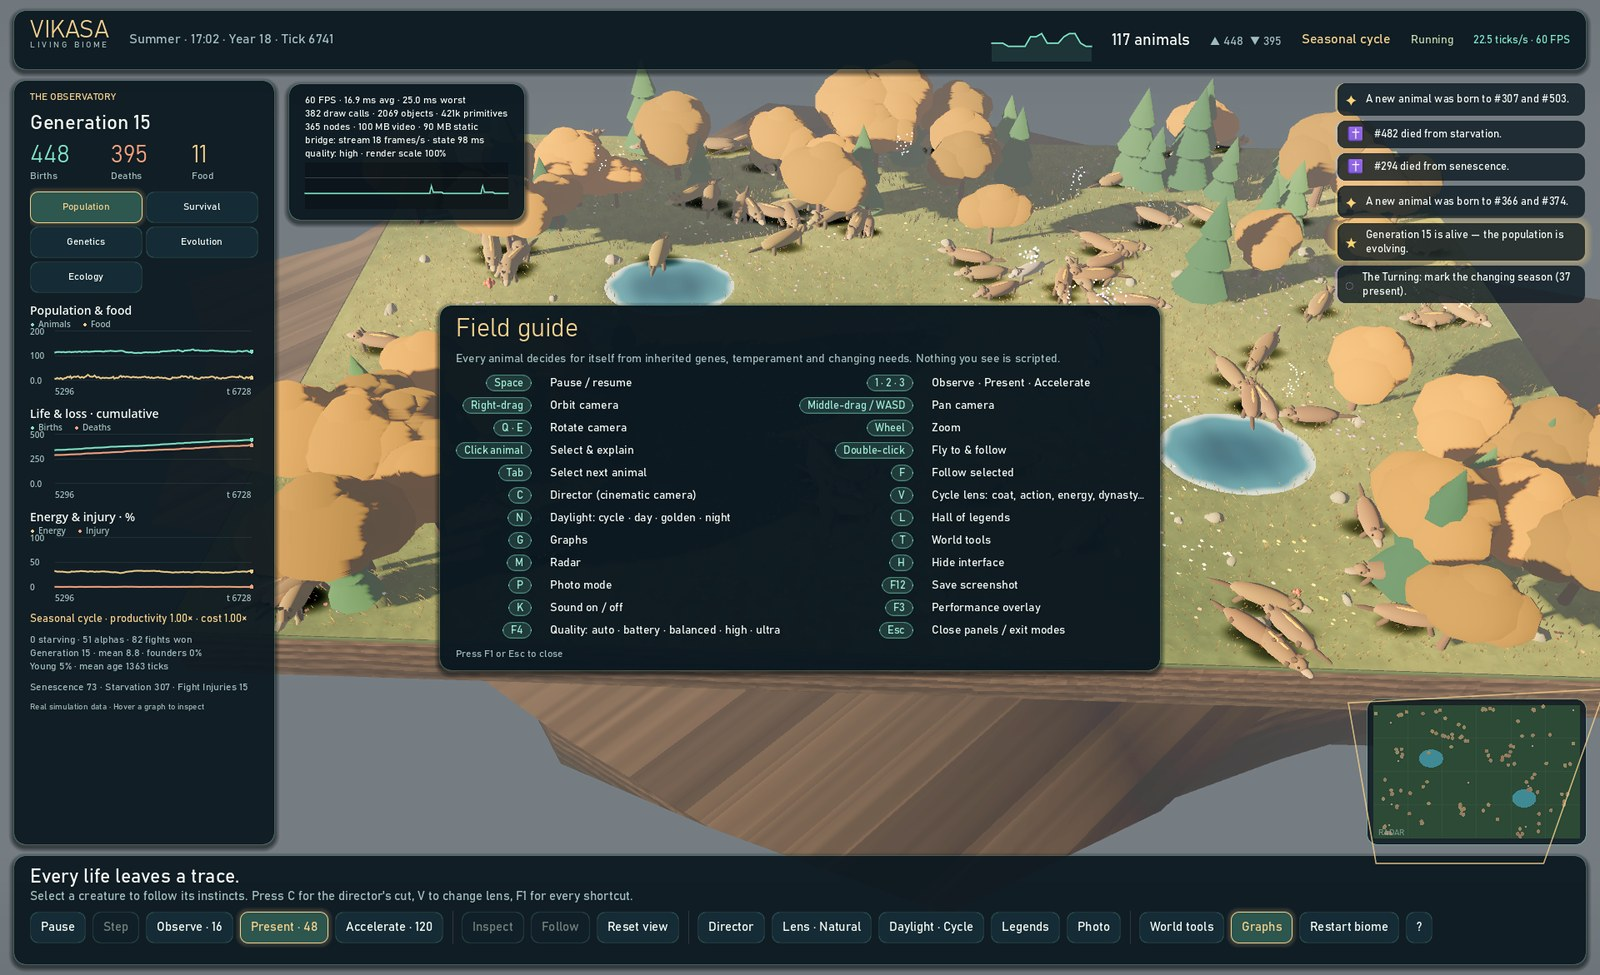
\includegraphics[width=0.6\textwidth]{showcase-help.jpg}
\caption{Field guide (F1) and the F3 performance overlay.}
\end{figure}

%===========================================================
\chapter{Local Application Server and API}
%===========================================================
\code{vikasa app}, \code{risk}, \code{plan} and \code{demo} serve one loopback
application on \code{http://127.0.0.1:8787}. The server refuses non-JSON and
cross-origin requests, and launch requests are whitelisted.

\begin{longtable}{p{2.1cm}p{5.4cm}p{6.9cm}}
\caption{Application server routes}\\
\toprule
Method & Path & Purpose \\
\midrule
\endfirsthead
GET & \code{/}, \code{/risk}, \code{/plan}, \code{/demo} & Home screen, Risk Checker, Planner, presenter hub. \\
GET & \code{/api/meta} & Places, presets, tolerance modes, SSPs, reference curve. \\
GET & \code{/api/estimate} & Instant estimate (\code{place}, \code{generation\_years}, \code{tolerance}, \code{ssp}). \\
POST/GET & \code{/api/live}, \code{/api/live/<id>} & Start and poll a live check. \\
GET/POST & \code{/api/plan/example}, \code{/api/plan} & Example watchlist; triage a pasted or uploaded CSV. \\
POST & \code{/api/watch} & Write a scenario world and open it in 3D. \\
POST & \code{/api/launch} & Launch \code{biome}, \code{biome-demo} or \code{climate-demo}. \\
GET/POST & \code{/api/godot}, \code{/api/stop-godot} & 3D window status; close it. \\
POST & \code{/api/fetch} & Download a new place from NASA POWER. \\
GET & \code{/api/stats}, \code{/api/version} & Live project statistics; version handshake. \\
GET & \code{/evidence/...} & The committed evidence report. \\
POST & \code{/api/quit} & Shut down every Vikasa process. \\
\bottomrule
\end{longtable}

%===========================================================
\chapter{Testing and Quality Assurance}
%===========================================================

\section{Test suite}
\code{pytest} collects 554 tests (with \code{--strict-markers --strict-config};
long stress tests are marked \code{slow}). Hypothesis is available in the
development extras for property-based testing.

\begin{longtable}{p{4.4cm}p{10.6cm}}
\caption{Test areas}\\
\toprule
Area & What is verified \\
\midrule
\endfirsthead
\code{tests/model/} & Genome bounds and immutability, crossover/mutation, diploid expression and meiosis, entities, spatial hash, 2D maths. \\
\code{tests/simulation/} & Engine tick order and invariants, reproducibility of identical seeds, behaviour drives/utilities/arbitration, Gompertz demography, habitat growth, diffusion conservation and ledgers. \\
\code{tests/analytics/} & Metrics, exact Price identities, evolutionary change, trait-space PCA and undefined cases. \\
\code{tests/io/} & Checkpoint round-trips, migration, strict rejection of corrupted data; export manifests. \\
\code{tests/experiments/} & Runner, contrast protocol validation, paired statistics, dashboard. \\
\code{tests/climate/} & Data parsing and provenance, forcing, engine coupling, protocol, analysis, Sobol on Ishigami, surrogate, assessment, report, CLI, risk screen (published verdicts), planner. \\
\code{tests/ui/}, \code{test\_bridge\_stream.py} & Pygame smoke tests; binary frame contract and stream. \\
\code{test\_cli.py}, \code{test\_config.py}, \code{test\_shortcut.py}, \code{test\_documentation.py} & CLI parsing, configuration validation, shortcut creation; documented scenarios load, every documented mode is in the CLI help, example results are audited, screenshots are real rendered images. \\
\bottomrule
\end{longtable}

\section{Godot headless checks}
\code{SceneContractSmoke}, \code{BehaviorPresentationSmoke}, \code{LocusChartSmoke}
and \code{DemoPilotSmoke} run headless. \code{PerfProbe} measures mean and p99 frame
time, slow-frame share, draw calls, node count and tier, with \code{--breakdown},
\code{--freeze}, \code{--no-state} and \code{--no-frames} isolation flags.
\code{ShowcaseCapture}, \code{PresentationCapture}, \code{WildlifeCapture} and
\code{MainCapture} regenerate documentation screenshots from real bridge states.

\section{Invariants}
\code{SimulationEngine.audit\_invariants} returns a list of violations, checked by
\code{stress}, \code{study}, \code{contrast} and the climate runs. It verifies that
dictionary keys match creature and resource IDs; motion state, energy and resource
state are finite; every creature lies inside the world; home centres, radii and
migration counters are valid; all six traits lie within configured bounds; diploid
genotypes are valid, require a diploid architecture and match the expressed
phenotype; thermal optima are valid and exist only with climate forcing; external
food inputs and their intervention history are finite and consistent; and the
habitat's update count equals the engine tick. Study reports additionally check
the population identity living $=$ founders $+$ births $-$ deaths, and checkpoint
loading verifies reservoir ledgers and Price identities.

%===========================================================
\chapter{Performance}
%===========================================================

\section{3D client}
Measured on an Intel Core i5-1335U with Iris Xe graphics, $1920\times1200$ at
59\,Hz, Windows 11, Godot 4 Compatibility renderer, showcase seed 2026 with about
110--170 animals.

\begin{table}[htbp]
\centering
\caption{Living Biome before and after version 2.0}
\begin{tabularx}{\textwidth}{lLL}
\toprule
Measure & Before (v1.1) & After (v2.0) \\
\midrule
Frame rate with vsync & 13--14 FPS & \textbf{59.6--59.9 FPS} at high \\
Uncapped, full interface & 35--152 FPS, p99 36--157 ms & 98--105 FPS high; 149 FPS balanced \\
Frames over 25 ms (vsync) & --- & 0.1--0.4\% (p99 21--22 ms, plugged in) \\
Draw calls / scene nodes & $\sim$1{,}700--2{,}450 / $\sim$3{,}000--3{,}600 & $\sim$20 for the 3D world ($\sim$300 with UI) / 365 \\
Explanatory document & 180--680 KB every 0.16--0.45 s & $\sim$35 KB every 0.4 s \\
State request latency & 49 ms median & 12 ms median \\
\bottomrule
\end{tabularx}
\end{table}

On battery, vsync'd rendering was near 45 FPS; after the battery-aware pacing
change \code{auto} settled on balanced, unlocked, at 94.5 FPS (p99 29\,ms). With the
complete 3D window open, this laptop sustained about 43 ticks/s in a 12-second
Accelerate sample; the 120 ticks/s setting is a ceiling, not a guarantee.

\section{Engine}
A profile of spatial-biome seed 2026 (150 ticks after 150 warm-up) attributed
2.54\,s to spatial rebuilding, 2.42\,s to insertion and 1.81\,s to radius queries
out of 13.72 profiled seconds. The spatial hash was then changed to validate each
position cloud with one NumPy reduction and keep copied scalar coordinates.
\code{tools/benchmark\_spatial.py} loads the historical index from Git into an
isolated namespace, alternates run order, and requires identical full checkpoint
digests at both boundaries.

\begin{table}[htbp]
\centering
\caption{Guarded spatial-index benchmark (Python 3.12.14, NumPy 2.5.3)}
\begin{tabular}{lccc}
\toprule
Seed & Historical ticks/s & Optimised ticks/s & Ratio \\
\midrule
2026 & 20.03 & 23.97 & 1.197 \\
7 & 21.72 & 24.94 & 1.148 \\
41 & 20.85 & 23.83 & 1.143 \\
\bottomrule
\end{tabular}
\end{table}
All pairs matched digests and reported no invariant errors: a local 14--20\%
improvement with unchanged biology, not a universal guarantee.
